\documentclass[10pt,a4paper,twoside]{article}
\usepackage{a4wide}
\linespread{1.359140914229522617680} 
\usepackage[utf8]{inputenc}
\usepackage[german]{babel}
\usepackage{bibgerm}
\usepackage{amssymb}
\usepackage{graphicx}
\usepackage{hyperref}
\usepackage{placeins}
\hypersetup{
%    bookmarks=true,
    pdftoolbar=true,
    pdfmenubar=true,
    pdffitwindow=false,
    pdfstartview={FitH},
    pdftitle={Das Nizza Modell},
    pdfauthor={Michael F. Sch\"onitzer},
    pdfsubject={Das Nizza Modell},
    pdfkeywords={Nizza-Modell},
    pdfnewwindow=true,
    colorlinks=true,
    linkcolor=black,
    citecolor=black,
    filecolor=black,
    urlcolor=blue
}
% Experminentel, bis ich mich für was entscheiden habe.
\usepackage[super,nospace]{cite}
\makeatletter
\def\@citess#1{\textsuperscript{[#1]}}
\makeatother
%\renewcommand{\thefootnote}{\fnsymbol{footnote}}

% Bilder & Tabellen ausblenden
\usepackage{comment}
\renewenvironment{figure}{}{}
\renewenvironment{table}{}{}
\excludecomment{figure}
\excludecomment{table} 
 
\author{Michael F. Schönitzer}
\title{Das Nizza Modell}

\newcommand{\refsec}[1]{siehe Kapitel \ref{#1}}
\newcommand{\degree}{$^\circ$}

\begin{document}
\maketitle

\section{Einleitung}
Im Jahr 2005 veröffentlichen Gomes, Levison, Morbidelli und Tsiganis drei Nature-Artikel\cite{Gomes2005}\cite{Tsiganis2005}\cite{Morbidelli2005} %Reihenfolge
in denen sie ein neues Modell für die Migration der Riesenplaneten unseres Sonnensystem vorstellten. Dieses Modell ist außerordentlich erfolgreich und wird Nizza-Modell genannt, da die Autoren zu besagter Zeit am Observatoire de la Côte d’Azur in Nizza arbeiteten.

Das Nizza-Modell betrachtet das Sonnensystem nachdem sich die Gasscheibe bereits aufgelöst hat, das Sonnensystem besteht nun aus der Sonne, den Planeten und einer Scheibe von Planetesimalen. Das Modell geht in Übereinstimmung mit Planetenentstehungsmodellen %wirklich?
davon aus, dass die Planeten damals nahezu kreisförmige, kompakte Orbits hatten.

Aus dieser Scheibe werden von den Planeten\footnote{Sofern nicht anderes angegeben, betrachten wir im folgenden immer nur die vier Gasriesen Jupiter, Saturn, Uranus \& Neptun. Die terrestrischen Planten sind aufgrund der geringen Masse vernachlässigbar.} immer wieder einzelne Planetesimale gestreut oder akkretirt. % Akkretiert? 
Dabei kommt es durch die Impulsübertrag zu einer Änderung der Planetenorbits\cite{Tsiganis2005},
wodurch Saturn, Uranus und Neptun langsam nach außen wandern, während Jupiter langsam nach innen wandert\cite{Tsiganis2005}\cite{Hahn1999}. % Hahn nicht gelesen
Mit der Zeit kommen sich die Planeten durch die Migration näher und es kommt zu einer Resonanz,
welche zu einer schlagartigen Erhöhung der Exzentrizitäten der Umlaufbahnen von Jupiter und Saturn, auf Werte die mit den heutigen vergleichbar sind, führt.
Die Planeten Saturn Uranus und Neptun kommen sich gegenseitig und der Scheibe aus Planetesimalen nahe. Dadurch werden die Planetesimale praktisch schlagartig zerstreut, das System wird instabil und ein Teil der Planetesimale fliegt in das innere Planetensystem und löst dort das Late Heavy Bombardment aus.

Nach etwa hundert Millionen Jahren erreichen die Planeten schließlich ihre heutigen Entfernungen, ihre Exzentizitäten werden gedämpft und das System stabilisiert sich wieder. Die übriggebliebenen Planetesimale bilden die heutigen transneptunischen Objekte.

Neben den Plantenorbits (\refsec{Orbits}), dem Late Heavy Bombardment (\refsec{LHB}) und dem Kuipergürtel (\refsec{Kuiper}), kann das Modell, wie wir sehen werden, auch die Trojaner (\refsec{Trojaner}), die irregulären Monde (\refsec{Monde}) und die Achse des Uranus (\refsec{Uranusachse}) zumindest prinzipiell erklären.
Abschließend werden wir uns mit einer möglichen Erweiterung des Nizzamodells um zusätzliche Anfangsplaneten beschäftigen (\refsec{mehrPlaneten}).

\FloatBarrier
\section{Das Nizza-Modell}\label{Orbits}
In diesem Kapitel werden wir das Nizzamodell wie in der ursprünglichen Arbeit\cite{Tsiganis2005} beschrieben erläutern. %superbäh

In der Simulation berücksichtigten die Forscher dabei die vier Riesenplaneten auf sehr kompakten Orbits, sowie eine Scheibe aus Planetesimalen im Gravitationsfeld der Sonne. % Bäh: Forscher?
Dies ist ein plausibler Ausgangszustand für die Situation nachdem der Sonnenwind die Gaswolke %Sonnenwind, Gaswolke?
zerstreut hat. % bäh: formulierung
Als Anfangsparameter wählten Tsiganis et. al in den Simulationen für die große Halbachse des Jupiterorbits $a_J = 5,45 AU$. Saturn wurde wenige Zehntel AU vor der bei $a_{1:2} = 8,65 AU$ gelegenen 1:2-MMR gesetzt\cite{Tsiganis2005}.% F***: die erklärung von MMRs ist erst weiter unten
Das Saturn weiter innen als auf der zu Jupiter resonanten Bahn war ist auch eine notwendige Bedingung, da es anderenfalls schon zu Zeiten der Gasscheibe eine starke Migration durch die Wechselwirkung mit dieser gegeben hätte\cite{Levison2008}. %O-Zitat, klarer
Die Orbitalverteilung der transneptunischen Objekte lässt darauf schließen, dass Neptuns Migration innerhalb von 20 AU begonnen hat\cite{Tsiganis2005}.
Die beiden Eisplaneten wurden in den Simulationen von der Gruppe von Tsiganis mit großen Halbachsen von 11-13 AU respektive 13,5-17 AU, mit einem Mindestabstand von 2 AU gestartet.
Die Planetenorbits waren, wie von den Planetenentstehungsmodellen gefordert, % formulierung, Quelle
nahezu kreisförmig und coplanar ($e, i \approx 10^{-3}$).

Die Planetisimalenscheibe – ein Überbleibsel der Planetenentstehung – begann 1.5 AU hinter dem Orbit des zweiten Eisplaneten und reichte bis zu einer Entfernung von 30-35 AU hinaus\cite{Tsiganis2005}\cite{Levison2008}. Sie bestand aus 1000-5000 gleich schweren Brocken, mit einer Gesamtmasse von 30 bis 50 Erdmassen. %Ausdehnung steht oben, runter?
Die Flächendichte der Scheibe wurde in den Simulationen linear mit dem Sonnenabstand abfallend gewählt. In einigen Simulationen wurde eine dynamisch "heiße"\ Scheibe in anderem eine "dynamisch kalte"\ Scheibe gewählt, wobei mit dynamisch heiß gemeint ist, dass Exzentrizität und Inklination relativ groß waren: $e \approx \sin i \approx 0.05 $, im Vergleich zu $e \approx \sin i \approx 10^{-3} $ im kalten Fall.\cite{Tsiganis2005}
Die Eigengravitation der Scheibe wurde in den Simulationen ignoriert\cite{Tsiganis2005}.
Die Simulationen wurden mit zwei verschiedenen symplektischen N-Körper Codecs durchgeführt: MERCURY von John Chambers und SyMBA, einer Erweiterung des von Hal Levison und Martin Duncan entwickeltem SWIFT.
% http://www.boulder.swri.edu/~hal/swift.html
% http://www.arm.ac.uk/~jec/
Der Zeitschritt betrug zwischen einem viertel und einem halben Jahr.\cite{Tsiganis2005} % REALY?

Aus dieser Scheibe werden von den Planeten immer wieder einzelne Planetesimale gestreut oder akkretirt. Dabei kommt es durch die Impulsübertrag zu einer Änderung der Planetenorbits\cite{Tsiganis2005}. %Kinderkacke
Die Simulationen zeigen, dass Saturn, Uranus und Neptun langsam nach außen wandern, während Jupiter langsam nach innen wandert\cite{Tsiganis2005}\cite{Hahn1999}. % Hahn nicht gelesen

\begin{figure}[tbn]
\includegraphics[scale=1]{img/Tsiganis2005-1.pdf}
\caption{•}
\end{figure}
Während der Migration werden die Exzentrizitäten durch den gravitativen Einfluss der Planetesimale, bekannt als dynamische Reibung, gedämpft.\cite{Tsiganis2005}
Mit der Zeit kommen die Planeten sich durch die Migration näher, so dass Ressonanzen (englisch mean motion resonance, MMR) auftreten.
Man betrachtet im Nizza-Modell die 2:1-Resonanz zwischen Jupiter und Staturn, welche nach ein paar hundert Millionen Jahren auftritt.
Bei einer MMR handelt es sich um den Fall, dass die Umlaufdauern zweier Planeten im Verhältnis zweier kleiner natürlicher Zahlen steht. In der hier relevanten 2:1-MMR zwischen Jupiter und Saturn, läuft also Jupiter genau zweimal um die Sonne, während Saturn in der selben Zeit genau einmal seinen Orbit durchlauft, die Planeten "begegnen"\ sich also immer am selben Ort. %Nochmal Prüfen
Die 2:1-Resonanz zwischen Jupiter und Saturn ist die stärkste Resonanz. % einbauen
Die Autoren testeten auch Anfangsbedingungen, welche zum Auftreten von anderen MMRs führten. Doch weder die 2:3 MMR zwischen Saturn und dem inneren Eisriesen, noch die 1:2 MMR zwischen den beiden Eisriesen waren stark genug um die Bahn von Jupiter zu beeinflussen\cite{Tsiganis2005}. % Tsiganis2005 hats noch genauer
Die Resonanz für zu einer schlagartigen Erhöhung der Exzentrizitäten der Umlaufbahnen von Jupiter und Saturn, auf Werte die mit den heutigen vergleichbar sind. %genauer erklären?
Dadurch stören Jupiter und Saturn die Eisplanenten, so dass auch deren Exzentrizitäten abhängig von den genauen Anfangsparametern (Massen und großen Halbachsen der Planeten) mehr oder weniger stark anwachsen\cite{Tsiganis2005}.
Da die Planetenorbits sehr dicht aneinander liegen, führen die hohen Exzentrizitäten zu überschneidenden Bahnen\cite{Tsiganis2005}, es kommt dadurch zu Begegnungen von Planeten. %Bäh: Begegnungen
Dies hat wiederum zwei Effekte: die Inklinationen der Planeten wächst um $1^\circ-7^\circ$ und die Eisriesen werden hinaus in die Planetesimalscheibe gestreut,
wodurch nun schlagartig eine große Menge an Planetesimalen ins Innere gestreut werden und sich folglich die Migrationsrate drastisch erhöht\cite{Tsiganis2005}.
Die große Anzahl an kleinen Objekten im Bereich der Planetenbahnen, führt jedoch zu dynamischer Reibung, wodurch die Exzentrizitäten und Inklinationen wieder langsam sinken und sich das System somit wieder stabilisiert\cite{Tsiganis2005}.
Wenn die Planetesimalscheibe fast vollständig zerstreut ist, stoppt die Migration der Planeten und sie erreichen ihre endgültigen Bahnen\cite{Tsiganis2005}.

\newcommand{\AU}{\;\mathrm{AU}}
\newcommand{\DII}{\Delta a_{I_1,I_2}}
\newcommand{\DSI}{\Delta a_{S,I_1}} % Formeln, nicht kursiv
Diese hängen von dem Verhalten des Systems zum Zeitpunkt direkt nach der Resonanz ab. In den 43 Simulationen in \cite{Tsiganis2005} zeigte sich, dass von den zahlreichen Anfangsparametern der Abstand der Eisriesen $\DII$ und vor allem der Abstand zwischen Saturn und dem inneren Eisriesen $\DSI$ die größten Auswirkungen haben\cite{Tsiganis2005}. %Diese spezifizieren?
Wie oben schon erwähnt, wurden für $\DII$ Werte zwischen etwa zwei und sechs AU verwendet, während die Werte von $\DSI$ zwischen ~2.5 und ~5 AU betrugen\cite{Tsiganis2005}.
Wählt man den Abstand zwischen Saturn und dem ersten Eisplaneten klein, so steigt die Wahrscheinlichkeit, dass einer der Eisplaneten von Saturn auf ein die Jupiterbahn kreuzendes Orbit gestreut wird und dann von Jupiter aus dem System geschleudert wird. Für $\DSI \le 3 \AU $ geschah dies in 14 der 43 Simulationen (33\%).
Wählt man den Abstand hingegen sehr groß ($\DSI \approx 5 \AU$), so ist das System möglicherweise nicht mehr kompakt genug, so dass überhaupt keine Begegnungen von Planeten stattfinden. %bäh: Begegnungen

\begin{figure}[tbn]
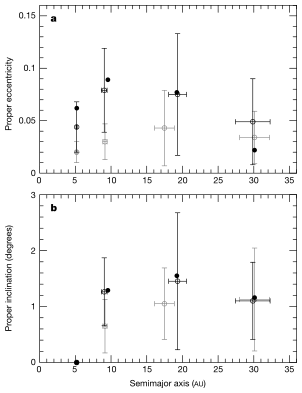
\includegraphics[scale=1]{img/Tsiganis2005-2.pdf}
\caption{•}
\end{figure}
Für die restlichen Fälle, welche allesamt nach einer wie oben beschriebenen Migrationsphase wieder zur Ruhe kommen %bäh: zu Ruhe kommen
gilt, dass es für Abstände $\DII \ge 3.5 \AU$ zwar zu Interaktionen der beiden Eisplaneten unter einander, nicht jedoch zwischen einem Eisriesen und Saturn kommt, während es in Simulationen mit kleinerem $\DII$ auch zu solchen kommt. In Übereinstimmung mit der Originalveröffentlichung, bezeichnen wir erstere Art von Simulationen als Klasse A und letztere als Klasse B\footnote{Die beiden Fälle in der es zu keiner Begegnung kam, wurden aus mir nicht ganz nachvollziehbaren Gründen nicht ausgeschlossen sondern zur Klasse A gerechnet.}, Nesvorný et al. bezeichneten Klasse A als Malhotra Klasse (MA) und Klasse B als 'direct emplacement`-Klasse (DE)\cite{Nesvorny2007}. %Malhotra zitieren?

Bei Klasse B wird Neptun durch Uranus direkt fast auf seine Endgültige Entfernung geschleudert und anschließend wird die Exzentrizität durch dynamische Reibung in der Planetesimalscheibe verringert\cite{Nesvorny2007}. Somit ist die Zeitdauer der Phase der Schnellen Migration bei dieser Klasse kürzer\cite{Tsiganis2005}. Auch führt diese Art der Dynamik dazu, dass die Exzentrizität weniger stark abnimmt\cite{Tsiganis2005}.
Bei den Simulationen der Klasse A wird Neptun auf eine etwa $22-25 \AU$ von der Sonne entfernte Umlaufbahn geschleudert und Migriert dann langsamer innerhalb der Planetesimalscheibe auf seine endgültige Position\cite{Tsiganis2005}.
14 der Simulationen waren vom Typ B, 15 vom Typ A. % Satz häßlich
Die Durchschnittswerte und Standardabweichungen für die großen Halbachsen, Exzentrizitäten und Inklinationen der Planeten von beiden Gruppen sind in Grafik \ref{AvsB} aufgetragen. Wie man sieht stimmen die Resultate beider Klassen fast mit den tatsächlich beobachten Werten überein, im Fall der Klasse B ist die Übereinstimmung jedoch deutlich größer – hier liegen sogar alle Messewerte innerhalb nur einer Standardabweichung um den Mittelpunkt\cite{Tsiganis2005} – Klasse A hat ist etwas schlechter, insbesondere sind die Exzentrizitäten von Saturn und Uranus deutlich zu klein\cite{Nesvorny2007}\cite{Tsiganis2005}. 
Dies stellt einen bedeutenden Erfolg des Modells dar und hebt sich von vorhergehenden Modellen ab.
So hatte zum Beispiel das Vorgängermodell von Gomes, Morbidelli und Levinson \cite{Gomes2004} %Namen prüfen
das Problem zwar vorsagen zu können, dass Neptun eine große Halbachse von etwa 30 AU hat, jedoch wart die Uranusbahn dabei zu dicht an der Sonne.
Die großen Halbachsen der Eisriesen für die Klasse B betragen im Nizza-Modell hingegen $a_U = 19,3 \pm 1,3 \AU$ und $a_N = 29,9 \pm 2,4 \AU$, was mit den tatsächlichen Werten von $a_U = 19,2 \AU$ und $a_N = 30,1 \AU$ sehr gut übereinstimmt\cite{Tsiganis2005}.

Der finale Abstand zwischen Jupiter und Saturn hängt vor allem von der Masse der Materie %bäh: finale
die sie während der instabilen Phase streuen ab, welche wiederum von der Masse der Planetenscheibe abhängt\cite{Tsiganis2005}. % richtig?
Höhere Massen der Scheibe führen zwar zu stabileren Endsystemen, wird die Masse jedoch größer als $\approx (35-40) M_E$ wird der Abstand zwischen Jupiter und Saturn im fertigsimuliertem System zu groß\cite{Tsiganis2005} und wählt man eine Masse von $\approx 50 \AU$, so tritt zwischen Jupiter und Saturn zusätzlich auch eine 2:5 Resonanz auf und die dynamische Reibung wird so groß, dass Exzentrizitäten kleiner als in Realität ausfallen\cite{Tsiganis2005}.

Die dynamische Temperatur der Scheibe wirkt sich auf die Exzentrizitäten aus: Heißere Scheibe führen zu höheren Exzentrizitäten von Jupiter und Saturn. Die beobachtete Existenz von zahlreichen plutogroßen Transneptunischen Objekten spricht laut den Autoren für eine Scheibe mit der Dynamik der heißeren der beiden getesteten Scheiben\cite{Tsiganis2005}. % Tsiganis2005 zitiert hier Stern 1991

%Gemäß aktueller Planetenentstehungsmodelle sollten sich die Gasplaneten auf kreisförmigen coplanaren Orbits gebildet haben, jedoch 
%warum ein Migrationsmodell überhaupt von nöten ist.
%Darüberhinausgehend nimmt das Modell an, dass bei der Planetenentstehung eine Scheibe von Planetesimalen entstand, die von außerhalb der Planetenorbits bis hinaus zu einer Entfernung von 30-35 AU\cite{Tsiganis2005} reichte und eine Gesamtmasse von etwa 35 Erdmassen hatte. %Überprüfen, Quellen, Doppelung entfernen


\begin{figure}[tbn]
\includegraphics[scale=1]{img/Gomes2005-2.pdf}
\caption{•}
\end{figure}

\FloatBarrier
\section{Late Heavy Bombardment}\label{LHB}
Geologische Untersuchungen von Mondgestein zeigen, dass es 700 Millionen Jahre nach der Plantenentstehung
eine enorme Häufung von Einschlägen gab, man nenn dieses Ereignis das Late Heavy Bombardment (LHB) oder auf deutsch auch das Große Bombardement.
%% Genauere Erklärung, bessere Quelle!
Die Planetenentstehungsmodelle können eine solche Häufung zu einem so spätem Zeitpunkt nicht erklären.
Es gibt einige Modelle zur Erklärung des LHBs jedoch sind diese relativ gekünstelt und kein Notwendiger Bestandteil der ansonsten abgeschlossenen Beschreibung der Entwicklung des Sonnensystems.\cite{Gomes2005} %Andre Quelle, genauer?
Im Rahmen des Nizza-Modells liegt es natürlich nahe anzunehmen das LHB sei durch die während der Instabilitätsphase zerstreuten Teilchen der Planetesimalenscheibe entstanden. % bäh: Teilchen

Das die Planetesimalenscheibe aufgrund ihrer Sonnenentstehung vermutlich eisig war und sie wie wir in Kapitel \ref{Kuiper} sehen werden, der Ursprung der heutigen Transneptunisch Objekte war, kann man sie als Kometen bezeichnen\cite{Gomes2005}. % wohin damit??

\begin{figure}[tbn]
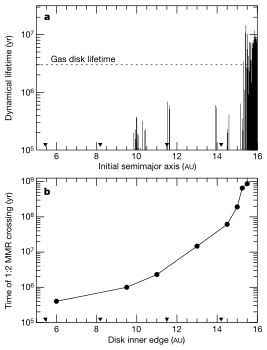
\includegraphics[scale=1]{img/Gomes2005-1.pdf}
\caption{•}
\end{figure}
%Bei folgenden Abschnitten bin ich mir noch nicht ganz sicher.
In anderen, ähnlichen Modellen – einschließlich frühen Versionen des Nizza-Modells – hatte man das Problem, dass die schnelle, durch das Streuen von Planetesimalen bedingte, Migration unmittelbar nach Simulationsbeginn eintrat und man somit nicht erklären konnte warum das LHB erst nach etwa 700 Myr stattfand.
Dies lag jedoch an einer falschen Startbedingung: Man hatte hierbei die Planetesimalen in die direkte Umgebung zu den Planeten gesetzt, was zwar zu einer gewünschten Migration führt, jedoch eine unnatürliche Startsituation ist,
denn es ist davon auszugehen, das die Migration durch Interaktion mit den Planetesimalen zum Zeitpunkt als das System noch in der Gasscheibe eingebettet war, im Vergleich zur Migration durch Interaktion mit der Gasscheibe vernachlässigbar ist.
Deshalb sollte die Anfangsbedingung des Nizzamodells gerade der Zustand sein, in welchem sich das Sonnensystem direkt nach dem Auflösen der Gasscheibe befand. Betrachten wir also nur die Migration nach dem Auflösen der Gasscheibe, so sollten alle zum Startzeitpunkt existierenden Planetesimale sich auf Orbits befinden, die stabil genug sind um bis zu diesem Zeitpunkt überhaupt überlebt zu haben. %Doppelung, am Anfang des Satzes zum Ende des letzten
Die Planetesimalscheibe sollte also nur Teilchen auf Bahnen haben deren dynamische Lebenszeit größer als die Lebensdauer der Gasscheibe ist.\cite{Gomes2005} Berücksichtigt man diese Bedingung, erhält man die schon in Kapitel \ref{Orbits} vorgegriffene Anfangsbedingung, das die Planetesimalscheibe hinter dem letzten Planeten beginnt, und zwar hinter etwa 15,3 AU.\cite{Gomes2005}

Die anfängliche Migrationsrate hängt nun von der Rate ab, mit welcher Planetesimale auf Planetenorbits schneidende Orbits gestreut werden. Der Zeitdauer bis zum auftreten der MMR hängt schließlich von den folgenden Parametern ab:
1. Dem Anfangsabstand zur Ressonanz, 2. der Dichte der Scheibe am inneren Rand und 3. der Abstand zwischen dem inneren Rand der Scheibe und dem äußeren Eisplaneten.\cite{Gomes2005}

In acht Simulationen untersuchten sie die Abhängigkeit des Ressonanzzeitpunktes in Abhängigkeit von der Position des inneren Rands der Planetesimalscheibe, bei ansonsten gleichen Parametern – inklusive gleicher Scheibenmasse und Dichte. Wie in Bild \ref{Bildfehlt} zu sehen ist, steigt die Zeit stark mit der Entfernung des inneren Rands an. Für große Werte $\gtrsim 15,3 \AU$ wie wir sie oben erhalten haben, tritt die Resonanz 192 bis 880 Millionen Jahre nach beginn der Simulation auf, was zum Zeitpunkt des LHB passen würde.\cite{Gomes2005} % Achtung: nach beginn der Simulation, nicht nach Planetenentstehung wie oben.
Durch zusätzliche Variation anderer Parameter konnte das Eintreten der Resonanz auf bis zu 1,1 Milliarden Jahre\cite{Gomes2005} verzögert werden – somit ist klar, dass das später Auftreten des großen Bombardements bei geeigneter Parameterwahl kein Problem bei Erklärung durch das Nizzamodell ist.

Als zweite wichtige Überprüfung, schauten sich die Wissenschaftler die Masse des auf den Mond treffenden Materials an. Bei den Simulationen waren dies etwa $9 \cdot 10^{21} \mathrm{g}$, davon trafen 50\% den Mond in den ersten 3,7 Millionen Jahren, 90\% in den ersten 29 Millionen Jahren. Das Bombardement fand demnach während einer relativ kurzen Zeitspanne statt. Die dabei durchschnittlich auf dem Mond treffende Gesamtmasse wurde auf $\left(8,4 \pm 0,3\right) \cdot 10^{21} \mathrm{g}$ bestimmt\cite{Gomes2005}.

Hinzukommt, dass es bei der Migration von Jupiter und Saturn von ihrer Position in der 2:1-MMR zu ihren heutigen Orbits zu einer weiteren Art von Resonanzen – die sogenannten Secular resonances treten auf wenn die orbitale Präzession zweiter Körper synchronisiert sind.\footnote{Ein deutscher Name ist mir nicht bekannt.} – % besser erklären was das ist!
kommt, welche über den Asteroidengürtel streifen. % bäh: streifen
Durch diese können Asteroiden Orbits mit so großen Exzentrizitäten und Inklinationen erhalten, so das diese bis ins innere Sonnensystem reichen. Wir müssen also die Masse der Asteroiden bestimmen, welche zusätzlich zu den Planetesimalen % die man als Kometen betrachten kann… <– hier oder wo anders?
mit dem Mond kollidieren.
Dafür führten die Autoren weitere numerische Simulationen durch in welchen sie die Auswirkungen von Sonne, Venus, Erde, Mars, Jupiter und Saturn auf den durch 1.000 masselose Teilchen gebildeten Asteroidengürtel untersuchten.
Die Migration der Gasriesen wurde dabei, durch das Hinzufügen von geeigneten Termen, künstlich hinzugefügt. % formulierung
Die große Halbachsen der Asteroiden betrugen dabei zwischen $2$ und $3,5 \AU$ und hatten Exzentrizitäten zwischen 0 und 0,3, sowie Inklinationen zwischen 0\degree und 30\degree – wobei das Perihel immer größer als $1,8 \AU$ und das Aphel immer kleiner als $4 \AU$ gewählt wurde. % Grund erläutern
Als Migrationsratten wurden in den Simulationen unterschiedliche Resultate der ursprünglichen Simulationen \refsec{Orbits} gewählt. %formulierung?

Gomes et al.\cite{Gomes2005} unterscheiden zwei Wege, auf welchen ein Asteroid auf ein die Erdbahn kreuzendes Orbit kommen kann. (1) Entweder es kommt zu einer Secular resonance zwischen der Periheldrehung des Körpers und der Periheldrehung Saturns, wodurch die Exzentrizitäten des Asteroiden steigen und er auf eine Erdbahnkreuzende Bahn gelangt, oder (2) sie werden im Asteroidengürtel dynamisch angeregt und wandern dann langsam aus dem Asteroidengürtel heraus\cite{Gomes2005}.
Weg (1) ist schneller, so das 50\% der Einschläge dieser Art bereits in den ersten 10 Myr (90\% in 30 Myr) stattfindet, während die Einschläge durch, auf letztere Art auf Kollisionskurs gebrachte, Asteroiden innerhalb von 50 Myr zu 50\% stattfanden (90\% in 150 Myr)\cite{Gomes2005}.
In den Simulationen von Gomes et al. war der zweite Typ häufiger, wobei dies wenig aussagt, da
die Häufigkeitsverteilung der beiden Wege vermutlich stark von den genauen Bedingungen abhängt\cite{Gomes2005} %genauer?
Die Masse an Asteroiden die den Mond gemäß diesen Simulationen trifft wurde auf $\left( 3-8 \right) \cdot 10^{21} \mathrm{g}$, % anderer strich statt minus? space
also einen ähnlich hohen Wert wie für die Planetesimale bestimmt – wobei die Unsicherheiten bei der Bestimmung der Masse der Asteroiden zu groß ist um ein Verhältnis zwischen den beiden Komponenten anzugeben. Auch ist noch nicht genau untersucht worden, inwieweit dieses Verhältnis eine Funktion von der Zeit und der Teilchengröße ist – so waren in diesen Simulationen die Planetesimale in den ersten 30 Millionen Jahren dominierend, die Asteroiden länger auf den Mond niederprasselten\cite{Gomes2005}.

Die Dauer des LHB beträgt in diesem Modell also zwischen 10 und 150 Millionen Jahren – eine genauere Bestimmung ist nicht möglich, da die Verhältnisse der beiden durch Asteroiden beigetragenen und des durch Planetesmiale beigetragenen Anteile sensibel von den genauen Anfangsparameter – insbesondere der genauen anfänglichen Struktur des Asteroidengültels – abhängen und daher nicht genauer bestimmt werden können\cite{Gomes2005}.

Vergleichen wir nun die Vorhersagen des Modells mit bekannten Messgrößen. Das Nizzamodell kann den für andere Modelle problematischen späten Zeitpunkt des Bombardements erklären. Auch die Menge des dabei auf den Mond eingebrachten Materials passt größenordnungsmäßig gut: So wurde aus der Anzahl und Größe der Mondkrater eine ungefähre Masse von $6 \cdot 10^{21} \mathrm{g}$ bestimmt, während die Simulationen $\left(8,4 \pm 0,3\right) \cdot 10^{21} \mathrm{g}$ an Planetesimalen und weitere $\left( 3-8 \right) \cdot 10^{21} \mathrm{g}$ an Asteroiden ergab.% [4] aus Gommes2005 zitieren!?
Das Modell sagt wie schön in Bild \ref{Bild_fehlt} zu sehen einen sehr plötzlichen Beginn des Bombardements voraus leider sind die bisher gemessenen Daten noch zu schlecht um dies zu überprüfen.
Das Nizza-Modell sagt voraus, dass sowohl Asteroiden, also auch Planetesimale auf dem Mond eingeschlagen sind, dies stimmt damit überein, dass kosmochemischen Analysen davon ausgehen, dass einige der Mondkrater durch Einschläge von Asteroiden geformt wurden.
Die Streuung von Asteroiden führt auch dazu, dass der Asteroidengürtel um einen Faktor von ungefähr 10 ausgedünnt wird, was zu bestehenden Modellen passt.  %Streuung Genauer!, Modelle citen!
Die Menge an Kometen, die während des LHB auf die Erde trafen ergibt sich im Nizzamodell zu $\approx 1,8 \cdot 10^{23} \mathrm{g}$ was etwa 6\% der heutigen Ozeanmasse beträgt und somit kompatibel zu der durch Isotopenhäufigkeit (D-zu-H-Verhältnis) bestimmten Obergrenze der durch Kometen eingebrachten Wassermenge\cite{Gomes2005}. % cite [13] in Gomes2005?!

Abschließend möchte ich noch darauf hinweisen, dass es neuere geologische Forschungen gibt, welche die Notwendigkeit der Existenz des Late Heavy Bombardments in Frage stellen\cite{Spudis2011}. % ausführlicher

\FloatBarrier
\section{Trojaner}\label{Trojaner}
Als Trojaner bezeichnet man Objekte, die auf dem selben Orbit wie ein Planet kreisen, jedoch um 60\degree vor- oder rückläufig bei den die Lagrangepunkten %L3 und L4? Schreibweiße
des Planeten.
Die Jupiter-Trojaner wurden in der Literatur häufig als Argument gegen das Auftreten der 1:2-MMR zwischen Jupiter und Saturn genannt. Das Überschreiten der Resonanz würde die Trojanerbahnen destabilisieren und die Trojanerpopulation vollständig auslöschen\cite{Morbidelli2005}. %O-Quelle
Morbidelli et al. zeigten dies ebenfalls mit einer Simulation, in welcher von 1,3 Millionen simulierten Trojanern kein einziger das Überschreiten der Resonanz überlebten\cite{Morbidelli2005}.

Man ging bisher davon aus, dass die Trojaner sich in der Nähe von Jupiter gebildet haben und als Jupiter wuchs entweder durch Kollisionen oder durch Reibung mit Gas %welches Gas
eingefangen wurden.
Dies hat jedoch das Problem, dass es unter anderem die große Inklinationsverteilung der Trojaner von bis zu 40 Grad erklären kann\cite{Morbidelli2005}. % welche anderen Probleme? O-Quelle
Da die Entwicklung von gravitativen Systemen zeit reversibel ist, %formulierung
können auf den selben Bahnen, auf welchen die Trojaner von ihren Co-Orbitalen Bahnen entkommen können, auch Objekte vorübergehend auf Trojanerbahnen gelangen.
Somit ergibt sich im Rahmen des Nizza-Modells ein alternatives Entstehungsmodell der Trojanerpopulationen: Während der Insablilitätsphase direkt nach Überquerung der Resonanz sind die Co-Orbitalbahnen um die Lagrangepunkte dynamisch offen, so dass eventuell vorhandene Trojaner entweichen können, genauso können jedoch die zahlreichen Planetesimale die im Nizza-Modell für die Migration verantwortlich sind durch diese Stellen wandern. % Stellen, wandern
Sobald sich die Jupiter- und Saturnbahnen weit genug von der Resonanz entfernt haben, wird die Region wieder stabil und die Objekte die zu diesem Zeitpunkt dort sind, sind von nun an dort gefangen und bilden die heute beobachtbaren Jupiter-Trojaner.

%Weggelassen: Erste QnD-Simulation
\newcommand{\PJS}{P_J/P_S}
Um dieses Konzept zu untersuchen, untersuchten sie zunächst wann genau es zum Verlust der Trojaner kommt, also wann die Co-Orbitalregionen offen sind. % untersuchen doppelt
Dazu führten Sie eine zweistufige Simulation durch. Im ersten Stritt wählten sie eine der ursprünglichen Simulationen, wobei sie – aus Gründen die später ersichtlich werden – eine Simulation mit relativ langsamer Migration wählten. %wird es von alleine offensichtlich?
In dieser Simulation maßen sie zu 40 Zeitpunkten das Verhältnis $\PJS$.
Nun simulierten sie für jeden dieser Werte das System um zu messen wie viele der Trojaner verloren gehen. Diese Simulationen umfassten jeweils die Sonne, Jupiter, Saturn (bei festem Verhältnis von $P_J/P_S$) sowie eine große Anzahl an maselosen Testteilchen und liefen über $2 \cdot 10^5 yr$.
Abbildung \ref{pic:fehlt} zeigt die Messwerte von $\PJS$ und den Anteil an Körpern welche den Simulationszeitraum überlebten. Man sieht zwei deutlich Minima, welche auch theoretisch erklärt werden können.
Bei $\PJS \approx 2.05$ tritt eine sekundäre 3:1 Resonanz zwischen $1/P_J-2/P_S$ und der Oszilationsfrequenz mit der die Trojaner um den Lagrangepunkt kreisen auf, diese führt zu einer vollständigen Destabilisierung der Gebietes und somit zum Verlust aller Trojaner.
Ein zweites Minimum ergibt sich durch die 2:1 Resonanz selbiger Größen und führt zum Verlust von etwa 70 \% der Trojaner.
Gemäß dem Zeitreversibilitätsprinzip sind dies auch die Zeiten, bei welchen ein Einfang von Planetesimalen wahrscheinlich ist.

Um nun die Theorie zu testen, führten sie zwei Simulationen durch,
wobei der als ''langsame Simulation`` bezeichnete Durchlauf die Geschwindigkeit von oben verwendet, während die ''schnelle Simulation`` eine drei mal schnellere Migration vorwies – somit stellen dies die langsamsten und schnellsten Migrationsfälle des Nizza-Modells dar, da dies hierfür der einzige wichtige Parameter ist, ist der Parameterraum abgedeckt. %hmm
Für den Zeitraum zwischen dem Beginn der ersten sekundär-Resonanz und dem Ende der zweiten, wurde ein konstanter Strom von Planetesimalen durch das System geschickt,
während die Planeten durch Hinzufügen von geeigneten Krafttermen in die Bewegungsgleichungen zur Migration gezwungen wurden.
Diese Testteilchen wurden dafür auf die Saturnbahn kreuzende Orbits, mit Exzentrizitäten und Inklinationen wie in den ursprünglichen Simulationen beobachtet, gesetzt und immer wenn ein Teilchen auf dem System verloren ging wurde es wieder auf seinem ursprünglichem Orbit gesetzt, so das die Teilchenanzahl immer konstant 1.163.000 betrug.
Insgesamt wurden in der langsamen Simulation 5.466.000 Teilchen entfernt und wieder eingefügt, 98 Teilchen endeten nach $1,2 \cdot 10^6$ Jahren – als sich die Co-Orbitalregionen stabilisiert haben – auf Trojaner bahnen.
Die wurden 19 mal kopiert und dann über weitere 10 Myr simuliert um ihre langzeitliche Stabilität zu testen.
Dabei wurden die Exzentrizitäten der Planeten durch Zusatzterme in den Bewegungsgleichungen wie im Nizza-Modell beobachtet gedämpf. Am Ende überlebten 266 Teilchen. Die gesamte Eingangseffizienz berechnet sich als $266/20/5466000 \approx 2,4 \cdot 10^{-6}$.
Bei der schnellen Migration wurde die Migrationsgeschwindigkeit verdreifacht und die Simulationszeit entsprechend gedrittelt, ansonsten blieb sie unverändert.
Bei dieser wurden insgesamt 2.773.000 Teilchen entfernt und wieder eingefügt und 174 Teilchen endeten auf Trojanerorbits. Sie wurden 9-mal geklont, 486 Teilchen überlebten am Ende.
Die Effizienz beträgt $486/10/2773000 \approx 1,8 \cdot 10^{-5}$.
In beiden Simulationen hatten etwa die Hälfte der der Trojaner Librationsamplituden $D$ von weniger als 30\degree – wie etwa 87\% der bekannten Trojaner.
Da viele der Trojaner mit größeren Librationsamplituden auf sehr großen Zeitskalen instabil sind passt dies mit der Beobachtung überein und für die weiteren Analysen wurden nur die Trojaner mit $D<30^\circ$ betrachtet.
Um zu überprüfen, ob die Vernachlässigung von Uranus und Neptun gerecht fertig % gerechtfertig
war, wurden einige der Simulationen unter Berücksichtigung der Effekte dieser wiederholt. % ausführlicher?!
Morbidelli et al. stellten fest, dass die Eisgiganten keinen Einfluss auf die Trojaner von Jupiter haben.
Aus den ursprünglichen Simulationen des Nizza-Modells, % ursprüngliche Simulationen
wurde die Masse der Planetesimale die während der Instabilitätsphase durch das Sonnensystem streifen, auf $\sim 3,4 M_\oplus$ bestimmt.
Die Masse der Trojaner mit Librationsamplitude von unter 30\degree berechnet sich als Produkt dieser Masse mit der Einfangseffizienz und einem Faktor $1/2$, da nur die Hälfte eine Librationsamplitude von $<30^\circ$ haben. Sie beträgt für die langsame Simulation $\sim4\cdot 10^{-6} M_E$ und für die schnelle Simulation $\sim 3\cdot 10^{-5}M_E$.
Beim Vergleich mit einem Literaturwert stellen Morbidelli et al. eine deutlich Differenz fest: der berechnete Wert ist um einen Faktor $\sim3-25$ kleiner als der Literaturwert.


\FloatBarrier
\section{reguläre und irreguläre Monde}\label{Monde}
\subsection{Hill-Sphäre}
Als Hill-Sphäre bezeichnet man das in erster Näherung kugelförmige Gebiet um einen Körper (in der Regel Planet) der einen zweiten (hier die Sonne) umkreist, in welchem die Gravitationskräfte des Planeten überwiegen. Dabei entspricht der Radius der Hill-Sphäre der Entfernung bis zum ersten beziehungsweise zweiten Lagrange-Punkt und berechnet sich zu\cite{Sheppard2005}:
\begin{equation}
r \approx a \sqrt[3]{\frac{m}{3 M}}
\end{equation}

\subsection{reguläre Monde}
Lorem ipsum

\subsection{irreguläre Monde}

\begin{figure}[tbn]
\includegraphics[scale=1]{img/Nesvorny2007-1.jpg}
\caption{ }
\end{figure}
\begin{figure}[tbn]
\includegraphics[scale=0.2]{img/Nesvorny2007-2.png}
\caption{•}
\end{figure}
\begin{figure}[tbn]
\includegraphics[scale=1]{img/Nesvorny2007-5.jpg}
\caption{•}
\end{figure}
\begin{figure}[tbn]
\includegraphics[scale=1]{img/Nesvorny2007-7.jpg}
\caption{•}
\end{figure}
\begin{figure}[tbn]
\includegraphics[scale=0.2]{img/Nesvorny2007-8.png}
\caption{•}
\end{figure}
\begin{figure}[tbn]
\includegraphics[scale=1]{img/Nesvorny2007-9.jpg}
\caption{•}
\end{figure}
Als irregulären Mond bezeichnet man einen natürlichen Satelliten auf Orbits die weit vom Planeten entfernt sind und eine starke Inklination haben\cite{Nesvorny2007}. %bessere Quelle
Häufig haben Sie auch retrograde Umlaufbahnen und große Exzentrizitäten\cite{Nesvorny2007}.
Inzwischen sind über 90 irreguläre Monde bei den Gasplaneten bekannt\cite{Nesvorny2007}\footnote{Andere Quelle sprechen von 113}. %bessere Zahl & Quelle
Während sich reguläre Satelliten unseres Wissens nach durch Akkretion aus der planetaren Gasscheibe gebildet haben, ist die Herkunft von irregulären Monden noch ungeklärt.
Sie müssen auf irgendeine Art von dem Planeten aus einem heliozentischem Orbit eingefangen sein worden, da eine Entstehung aus der planetaren Gasscheibe durch Akkretion wie bei den regulären Monden ist aus mehreren Gründen nicht möglich:
Sie sind von den regulären Trabanten räumlich zu stark getrennt um aus der selben Gasscheibe entstanden zu sein, per Akkretion können keine derartig großen Exzentrizitäten entstehen und vor allem können aus einer Gasscheibe keine retrogard umlaufende Planeten entstehen\cite{Nesvorny2007}. % besser formulieren!

Das System Sonne-Planet-einzufangender Körper reicht jedoch nicht aus, da das System Zeitreversibel ist und somit jeder Weg des Körpers von der heliozentischen Bahn zu der Planetenumlaufbahn auch wieder ein möglicher Weg zurück ist\cite{Nesvorny2007}. % formulierung
Es braucht also einen Mechanismus auf welche Weise ein Trabant dauerhaft eingefangen werden kann. Dazu wurde unter anderem vorgeschlagen, dass der Körper Energie durch den Reibung an, den Planeten umgebendes, Gas verliert. % die anderen 2 Modelle erwähnen?
Dieses Modell kann zwar einige der irregulären Moden von Jupiter erklären, nicht jedoch alle, da einige weiter entfernt als die Gasscheibe gereicht hat und auch auf die irregulären Monde von Neptun und Uranus lässt sich dieses Modell vermutlich nicht anwenden\cite{Nesvorny2007}. % genauer?
Migrationsmodelle, wie das Nizzamodell führen zu einem weiteren großen Problem für derartige "`gas-drag"'-Modelle. Kommt den so entstandenen irregulären Monden ein großer Planetesimal oder ein Planet zu nahe, werden sie äußerst effizient wieder aus dem System des Planeten gefegt\cite{Nesvorny2007}. Da im Nizzamodell sich die Planeten Saturn, Uranus und Neptun entsprechend nahe kommen, können die irregulären Monde die wir heute um diese Planeten sehen somit nicht aus der Zeit vor der Migration stammen\cite{Tsiganis2005}\cite{Nesvorny2007}, was für "`gas-drag"'-Modelle aber nötig wäre, da zum Zeitpunkt der Migration die Gasscheibe ja sich bereits aufgelöst hat\footnote{Es ist natürlich möglich, dass es früher andere "`Generationen"' von irregulären Monden gab, welche durch den Energieverlust in der Gasscheibe entstanden sind. }. % "`gas-drag"'-Modelle eindeutschen, definieren oder ohne Anführungszeichen?; pfuibäh: Fußnote wird derzeit über zwei Seiten verteilt

Eine weitere wichtige Eigenschaft der irregulären Monde sind ihre vielfältig variierten und keinem klaren Gradienten folgenden Farben. Würden die Monde aus lokalen Umgebung der Planeten stammen, müssten alle Monde eines Planeten eine ähnliche Farbe haben und die Farben der Monde müsst vom Sonnenabstand des Planeten abhängen\cite{Nesvorny2007}. Das beides nicht der Fall ist, ist ein Zeichen dafür, dass sie ein Mix aus Planetesimalen von ursprünglich ursprünglichen Orten sind. % formulierung, Quellen

Ein erster Ansatz um irreguläre Satelliten im Rahmen des Nizza-Modells zu erklären wurde 2006 von Ćuz und Gladman vorgestellt\cite{Cuk2006}. Dieser geht davon aus, dass irreguläre Monde auf relativ kleinen Bahnen durch "`gas-drag"'-Modelle entstehen und erst später ihre Bahnen durch die Instabilität des Systems anwächst. Dies konnte die oben angesprochenen Probleme der "`gas-drag"'-Modelle mit weit entfernten irregulären Monden zumindest bei Saturn – eingeschränkt auch bei Jupiter und Uranus – beheben\cite{Cuk2006}. % ausführlicher!?
Dieses Modell berücksichtigt jedoch nicht, dass es wie oben erwähnt im Nizza-Modell zu Annäherungen zwischen Planeten kommt, welche derartige irregulären Monde wieder aus ihrer Umlaufbahn werfen würde. Auch die anderen Erkenntnisse legen es nahe, dass die Monde erst während der Instabilitätsphase durch das Einfangen einiger der zahlreichen durch das Sonnensystem fliegenden Planetesimale entstanden. % bäh: fliegen, entstanden

Als Einfangmechanismus dient hierbei ein dritter massiver Körper,
% es fehlt die exchange reaction – rein, oder nicht? wenn ja, wo?
welcher sich dem Planeten auf weniger als einen Hillradiuses nähert und Körper, % Hillradius muss noch definiert und erklärt werden, vermutlich oben bei den regulären Monden.
welche zeitgleich ebenfalls durch den Hillradius fliegen anregen, so dass einige von ihnen auf stabilen Orbits enden. % bäh: enden
Da sich die Gasplaneten nach dem Eintreten der Resonanz näher kommen, während gleichzeitig eine große Anzahl an Planetesimalen das Sonnensystem durchstreift,
ergibt sich folgendes Bild: zwei Planeten kommen sich so nahe, dass Sie gegenseitig in den Hillradius des anderen eindringen,
einige der ebenfalls durch den Hillradius der Planeten fliegenden Planetesimale werden dadurch auf weit entfernten Bahnen um einen der Planeten mit großen Inklinationen eingefangen und % große Inklinationen?
kreisen nun als irreguläre Monde um den Planeten\cite{Nesvorny2007}.
% wohin damit:
In der Ausklingzeit des Nizza-Modells, als die Exzentrizitäten durch dynamische Reibung gedämpft werden und die Scheibe sich langsam leert, ist es möglich, dass die Bahnen der irregulären Monde durch vorbeifliegende besonders massive (vergleichbar mit Planeten) Planetesmiale noch einmal geändert werden. % bäh: die Klammer; Bahnen -> veralgm.??
Dies ist durchaus realistisch, da es keinen Grund gibt, warum sich außer den vier Riesenplaneten kein anderen großen Objekte gebildet haben sollen\cite{Nesvorny2007}. %bäh: 'Dies'
%

Wie oben beschrieben, modellierte die in Nizza ansässige Gruppe die Planetesimalscheibe als eine Scheibe von etwa 1000-5000 gleichschweren Körpern. Dies ist für die Makroskopische Beschreibung des Verhaltens ausreichend, jedoch ist zu erwarten, dass die Scheibe aus wesentlich mehr Teilchen mit unterschiedlichen Massen bestand.
Für die Analyse des hier beschriebenen Einfangprozesses der irregulären Monde, ist die Anzahl der Teilchen von zentraler Rolle, da die Wahrscheinlichkeit eines Einfangs offensichtlich mit der Anzahl der durch das Sonnensystem kreuzenden Planetesimalen steigt.
Die bei den ursprünglichen Simulationen gewählte Anzahl der Planetesimale ist viel zu gering um genügend Einfangprozesse zu beobachten um daraus Rückschlüsse auf die Orbits der eingefangenen irregulären Satelliten und die Effektivität des Einfangprozesses zu machen.
Auf der anderen Seite ist es -- aufgrund der limitierten Rechenzeit -- nicht möglich die Simulation mit der für die Analyse der Einfangprozesse notwendigen Genauigkeit zu berechnen, wenn die Teilchenzahl auch noch erhöht werden soll.
Um dies Problem zu lösen und die Effizienz dieses Einfangprozesses möglichst realistisch zu bestimmen, verwendeten Nesvorn\'{y} et al. ein mehrstufiges Verfahren: % Nesvorny als Quelle einbauen?

Für den ersten Satz von Simulationen, verwendeten Sie eine der ursprünglichen Simulationen von Gomes et al. als Ausgangspunkt\cite{Nesvorny2007}. % Gomes als Quelle einbauen?
Sie übernahmen die Positions- und Geschwindigkeitswerte aller Objekte zu einem Zeitpunkt kurz vor dem Eintreten der Resonanz und erhöhten dann die Teilchenanzahl der Planetesimalscheibe von einigen hundert auf 6868, %erklären warum nur einige hunder?
ohne die Gesamtmasse oder dynamischen Eigenschaften dieser zu ändern. 50 dieser Systeme, die sich nur durch die genauen Startwerte der einzelnen Planetesimale unterschieden wurden mit SyMBA über Zeitspannen von mindestens 130 Myr simuliert und dabei die Bahnen aufgezeichnet.
Von den sehr unterschiedlich ausfallenden Simulationen wurden im weiteren nur die 14 berücksichtigt, welche ein System lieferten, dass dem unsrigem halbwegs ähnlich war\cite{Nesvorny2007}. %genauer oder so ok?
Für diese Simulationen wurde alle Begegnungen von Planeten herausgesucht, bei welchen der Minimalabstand der Planeten kleiner als die Summe der Hillradien der Planten war. %bäh: herausgesucht

Im nächsten Schritt wurden dann die Positionen aller Körper von den Zeitpunkten der Begegnung $t_{enc}$ aus soweit in der Zeit zurückgerechnet, dass sie 5 AU weit von einander entfernt waren  $t_{enc} - \Delta t$\cite{Nesvorny2007}.
Dafür verwendeten sie nicht SyMBA sondern den flexiblere Bulirsch-Stoer Integrationsalgorithmus. % genauer? Quelle

Im dritten Teil der Simulationen wurden nun die berechneten Werte der Große Halbachsen, Exzentrizitäten und Inklinationen der Planetesimalen zum Zeitpunkt $t_{enc}-\Delta t$ verwendet um die Anzahl der Planetesimalen erneut stark zu erhöhen. Man generierte dafür $3 \cdot 10^6$ Teilchen auf zufallsverteilen Orbits, die der Orbitalverteilung der ursprünglichen Planetesimalen folgten und so gewählt waren, dass sie sich zum Zeitpunkt der Begegnung $t_{enc}$ in der nähe der sich begegnenden Planten sind. % Orbitalverteilung?, generieren oder hinzufügen?, formulierung
%Die Wahl dieser zufälligen Orbits ist möglich, da es zu diesem Zeitpunkt noch keine resonanten Strukturen in den Planetesimalen gibt.
Nun wurde das erweiterte System über einen Zeitraum von $2 \Delta t$ integriert und die Bahnen anschließend darauf untersucht welche der Planetesimale von einem Planeten eingefangen wurden. %formulierung
Eine weitere Integration erlaubte es zu testen, ob die eingefangene Körper stabile Orbits haben oder den Planeten wieder verlassen, bevor es zu einer erneuten Begegnung mit einem Planeten kommt.
Die Simulation der nächsten Planetenbegegnung erfolge identisch, nur dass hier zusätzlich auch die Teilchen berücksichtigt wurden, die bei der vorherigen Begegnung auf stabilen Orbits um einen Planeten endeten, berücksichtigt wurden.
Somit wurde berücksichtigt, dass Monde die derartig bei einer Drei-Körper-Begegnung eingefangen wurden möglicherweise bei einer erneuten Begegnung von Planeten wieder befreit werden können, sowie dass es möglich ist das ein ursprünglich von einem Planeten eingefangener Mond bei einer erneuten Begegnung zu einem anderen wechselt, oder zumindest seine Bahn verändert\cite{Nesvorny2007}. % zumindest rauswerfen
Abbildung \ref{pic:fehlt} zeigt beispielhaft anhand einer Simulation wie viele der endgültig von Uranus und Neptun gefangenen Körpern, bei welcher Begegnung eingefangen wurden.
Man erkennt, dass vor allem bei Uranus zahlreiche Generationen zur endgültigen Population beitragen, während bei Neptun nur einige duzend späte Generationen nennenswert beitragen.
Die Berücksichtigung dieser Effekte ist nicht nur für die korrekte Bestimmung der Einfangrate von Bedeutung, auch die Orbits der Monde unterschiedlicher Generationen unterscheiden sich, da die Planetesimalscheibe mit der Zeit immer stärker angeregt wird und die späteren Generationen somit aus einer stärker angeregten Scheibe stammen\cite{Nesvorny2007}.

Abschließend wurden alle nach der letzten Begegnung vorhandene, gebundene Teilchen mit einem weiteren Integrator % nennen?
auf ihre lang-zeitliche ($\geq 1 Myr$) Stabilität getestet %Formel fixen
und dabei die Durchschnittswerte von Großer Halbachse, Exzentrizität und Inklination der einzelnen Satelliten über die Zeit berechnet.
Für die anschließende Analyse wurden nur die bestehenden Monde betrachtet\cite{Nesvorny2007}. % einbauen, besseres Wort für: bestehenden
Bei der Analyse wird auch hier wider zwischen den beiden Klassen der Migrationsmodelle unterschieden \refsec{Orbits}.
Von den 14 erfolgreichen Simulationen vielen jeweils 6 auf die beiden Klassen und 2 weitere stellten Mischformen zwischen den beiden dar. Eine Besonderheit stellen die zu Simulationen Nummer 9 und 38 (Klasse B bzw. Mischform) dar, da es bei dieser anders als beim klassischem Nizza-Modell von Tsiganis et al.\cite{Tsiganis2005} auch zu Begegnungen mit Jupiter kam\cite{Nesvorny2007}.
Durchschnittlich kam es zu 383 Begegnungen von Planeten, wobei die Anzahl zwischen 55 und 1033 stark schwankte\cite{Nesvorny2007}.
Die Anzahl korreliert erwartungsgemäß mit der Gesamtdauer, die die Planeten auf sich kreuzenden Bahnen befinden und ist für die Klasse B höher (473 im Vergleich zu 169 bei Klasse A)\cite{Nesvorny2007}.
Mit durchschnittlich 345 Begegnungen gab es zwischen Uranus und Neptun die meisten Begegnungen\cite{Nesvorny2007}. %Doppelt
% Bei DE gab es mehr als bei DE <- Problem Klasse A hat per Definition garkeine. Wie rein, doch unterscheiden?
Die Begegnungen zischen Saturn und einem Eisgiganten ereigneten sich für gewöhnlich deutlich früher als die zwischen den Eisriesen.
Die Grafik \ref{pic:fehlt} zeigt die Minimalabstände und Geschwindigkeiten der 37 Saturn-Neptun- und 406 Uranus-Neptun-Begegnungen bei einer exemplarischen Simulation.
Das oszillierende Verhalten von der Geschwindigkeiten erklären die Autoren nicht\cite{Nesvorny2007}.
Auffällig ist dabei auch, dass es nach einer Zeitspanne von fast 800 Tausend Jahren noch einmal 4 Begegnungen gibt\cite{Nesvorny2007}.

Bild \ref{pic:fehlt} zeigt die Orbits der in einer der Simulationen von Klasse B erzeugten Uranus- und Neptun-Monde im Vergleich mit den heute real existierenden. % auch das Bild von Klasse A?
Die Werte für Uranus (\ref{pic:fehlt}a, \ref{pic:fehlt}b) stimmen bemerkenswert gut überein, wobei es auch hier zwei % nachzählen!
Abweichungen gibt. Zum einen ist die Verteilung der Inklinationen der retrograd laufenden Satelliten in Realität wie in der Grafik zu sehen dichter und etwas größer als in der Simulation, 
zum anderen – und das ist der größere Unterschied zwischen Modell und Realität – sind im Modell normal und rückwärtslaufende Trabanten etwa gleich häufig, während in Realität acht der neun Monde eine retrograde Bahn haben\cite{Nesvorny2007}.
Die zu niedrige Inklination könnte durch die Verwendung einer dynamisch kältereren Planetesimalscheibe oder durch eine Veränderung des Modells zugunsten der stärkeren Bedeutung früherer Generationen eingefangener Satelliten korrigiert werden\cite{Nesvorny2007}. %bäh: korrigiert werden
Die Asymmetrie zwischen normal und rückwärtslaufenden irregulären Monden ließe sich durch Kollisionen zwischen diesen beiden Gruppen erklären, welche in den Simulationen von Nesvorný nicht berücksichtigt wurden. So könnte Sycorax – der größte retrogarde, irreguläre Mond von Uranus (Durchmesser von etwa 190 km) – mehrere kleinere normalumlaufende Monde zerstört haben\cite{Nesvorny2007}. % Deutsches fachwort für normalumlaufend?
Für Neptun (\ref{pic:fehlt}c, \ref{pic:fehlt}d) stimmen die Resultate ebenfalls sehr gut überein, jedoch nur für 4 der 6 Monde, die Monde Neso und Psamathe haben deutlich größere Entfernungen von Neptun als die anderen\cite{Nesvorny2007}.
Simulationen der Klasse A können diese gar nicht erklären, für Simulationen der Klasse B waren derartig große Entfernungen zwar ungewöhnlich, kamen jedoch vor.
Der Unterschied zwischen den beiden Klassen bezüglich der maximal auftretenden großen Halbachsen liegt daran, dass die sogenannte 'evection ressonance` zu starken Instabilitäten für Bahnen mit $a \gtrsim \frac{1}{2} R_H$\cite{Nesvorny2007}. %O-Quelle
Der Hillradius eines Planeten wächst jedoch mit wachsender Entfernung von der Sonne und da bei der Klasse A Neptun zum Zeitpunkt der letzten Begegnung noch eine deutlich kleinere Bahn hat sind die großen Halbachsen seiner Monde auf $a < 0,26 \AU$ beschränkt\cite{Nesvorny2007}.
Auch dies ist ein Vorteil von Klasse B, wobei es auch Möglichkeiten gäbe Neso und Psamathe durch Streuung – zum Beispiel durch den Einfang von Triton – auf ihre heutigen Bahnen zu bringen. % Wo die Sonderrolle von Triton erläutern?
Fünf der 14 Simulationen erzeugten keine oder nur einen Trabanten um Saturn, bei den restlichen stimmten die Orbitalverteilung der Satelliten mit der der realen Planeten sehr gut überein, siehe \ref{pic:fehlt}\cite{Nesvorny2007}. % Bild rein?
In der schon oben erwähnten Simulation Nr. 9, in welcher es auch Planetenbegegnungen mit Jupiter gab, bekam auch dieser zahlreiche Trabanten (341 Stück), welche ebenfalls gut zu den beobachteten irregulären Monden passen. Dabei treten ähnliche Probleme wie bei Uranus auf, insbesondere was die zu kleinen Inklinationen der retrograden Monde angeht.
Zu Jupiter sollte noch angemerkt werden, dass bekannt ist, dass die meisten Monde auf rückläufigen Bahnen Fragmente von Kollisionen einiger größeren Monde waren, was den Vergleich der Orbits schwer macht\cite{Nesvorny2007}. %Nesvorny2004 als Quelle?

Nachdem die Teilchenanzahl in den Simulationen möglichst hoch gewählt wurde um möglichst genaue Aussagen über die Orbitale der Monde treffen zu können, % gefält mir so noch nicht
soll nun mit realistischeren Werten überprüft werden, inwieweit die Anzahl der durch das Modell erzeugten irregulären Monde mit der beobachteten übereinstimmt.
Dafür bestimmten Nesvorný et al. die Einfangwahrscheinlichkeit für einen Planetesimal durch einen Planeten.
Die Einfangquote eines Satelliten in einer Simulationen berechnet sich durch:
\begin{equation}
P_{\mathrm{capture}} = \sum\limits^{N_{enc}}_{j=1} \frac{N_{sat; j}}{N_{test}}\frac{N_{activ; j}}{N_{total}}
\end{equation} % eindeutschen!? besser setzen!
dabei ist $N_{enc}$ die Anzahl der Begegnungen mit anderen Planeten, $N_{sat;j}$ die zahl der bei der j-ten Begegnung erzeugten Satelliten, $N_{test} = 3 \cdot 10^6$ die zahl der jeweils injizierten Testteilchen, % injektieren oder injizierten?
$N_{active; j}$ ist die Anzahl an Teilchen die bei der Begegnung bei der ersten Simulation beteiligt waren und $N_{total} = 6868$ ist die Anzahl der in der ersten Simulation Anfangs verwendeten Planetesimale\cite{Nesvorny2007}. % bäh!
Die Durchschnittswerte der so berechneten Einfangswahrscheinlichkeit für Uranus und Neptun betragen $2,6 \cdot 10^{-7}$ beziehungsweise $5,4 \cdot 10^{-7}$, für Saturn und vor allem natürlich für Jupiter macht das betrachten des Durchschnittswertes aufgrund der großen Schwankungen wenig Sinn, hier verwendenden die Autoren die bei Simulation 9 auftretenden Maximalwerte von $8,5 \cdot 10^{-9}$ und $2,4 \cdot 10^{-8}$\cite{Nesvorny2007}.
Die Werte für $P_{\mathrm{capture;Saturn}}$ sind für Simulationen der Klasse B meist höher\cite{Nesvorny2007}. % steht das schon weiter oben?
Nachdem wir aus den Simulationen von Tsiganis et al. wissen, dass die Gesamtmasse der Planetesimalscheibe $\approx35M_\oplus$ betragen muss \refsec{Orbits}, % \oplus?
brauchen wir zur Bestimmung der Anzahl und Größe der irregulären Monde noch die size-frequency distribution (SFD) der Planetesimalscheibe. % size-frequency distribution übersetzen?
Da das Nizzamodell – wie wir in Kapitel \ref{Kuiper} besprechen werden – davon ausgeht, dass die Überreste der Planetesimalscheibe den heutigen Kuipergürtel darstellt und es nach dem LHB nur relativ wenige Veränderungen der SFD durch Kollisionen im Kuipergürtel gab, gehen die Autoren davon aus, dass die SFD des Kuipergürtels der der Planetesimalscheibe entspricht\cite{Nesvorny2007}.
Die SFD des Kuipergürtels entspricht in erster Näherung zwei Potenzfunktionen, für kleine Durchmesser folgt der SFD einer Potenzfunktion mit Exponenten $q_2 \approx 2-3$ während bei großen Durchmessern die SFD mit $q_1 \approx 4-4,5$ abfällt, wobei der Übergang bei etwa $D \approx 100$ Kilometern oder etwas darunter liegt\cite{Nesvorny2007}. %O-Quellen!?
Wählt man $q_2 = 2,75$, $q_1 = 4,25$ und $D = 100$ bei einer Planetesimalscheibenmasse von $35M_\oplus$ erhält man mit den  Einfangswahrscheinlichkeiten die in Abbildung \ref{pic:fehlt} rot gezeigten kumulierten SFDs für die eingefangenen Monde der vier Planeten. % ist das rot?
Beim Vergleich mit den schwarz eingezeichneten SFD der gemessenen irregulären Monde, % wirklich schwarz?
stellt man einige Abweichungen fest:
Uranus und Neptun haben es in Realität deutlich weniger irreguläre Monde als hier vorhergesagt, % Die Autoren verkaufen das sogar als Pro-Punkt, statt als Kontra-Punkt
Jupiter und Saturn haben deutlich zu viele kleine Monde und die SFD des Modells (gleich der des Kuipergürtels) ist allgemein für Mondradien von $D\gtrsim 10 \mathrm{km}$ deutlich steiler als in Realität (Exponent von $\approx2$\cite{Nesvorny2007}.
Dies sind einerseits große Diskrepanz zwischen Modell und Realität, jedoch wäre es ein deutlich größeres Problem, wenn das Modell zu wenige Monde erzeugen würde. So gibt es einige Effekte die diese Diskrepanzen erklären könnten:
\begin{itemize}
\item Die SFD der Planetesimalscheibe zum Zeitpunkt des Einfangs könnte doch anderes sein und sich erst später zu der des Kuipergürtels entwickeln.
So könnte Sie früher für flacher sein und sich erst später durch Kollisionen verändert haben. Dies würde sich jedoch nicht mit anderen Aussagen des Nizzamodells wie der Erklärung des LHBs oder der Existenz von Plutoiden vertragen, % erklären warum? Nesvorny2007 S.74 rechts oben
weshalb Nesvorný et al. dies als ungeeignete Erklärung ablehnen\cite{Nesvorny2007}.
Eine Reduzierung der Anzahl eingefangener Objekte wäre möglich, wenn ein größerer Massenanteil auf sehr kleine oder sehr große Objekte anfallen würde\cite{Nesvorny2007}. % anfallen, erklären warum von Bedeutung!, Diskussion
\item Durch Kollisionen zwischen Monden kann sich die SFD und die Anzahl der Monde verändern. Während des LHB durchdringen zahlreiche Planetesimale die Hillsphäre der Planeten und können dabei mit diese Kollidieren oder diese von ihrer Bahn bringen\cite{Nesvorny2007}. Durch diese Effekte könnten die meisten Monde zerstört werden und sich die SFD entsprechend ändern. Simulationen dies diese Effekte berücksichtigen wären möglich, sind mir jedoch nicht bekannt. % nochmal suchen!
\item Beim Einfang von Triton könnten Neptun-Monde verloren gegangen sein, was jedoch die Diskrepanz bei Uranus unberührt lassen würde\cite{Nesvorny2007}. % wo Tritonssonderrolle erklären?
\item Es könnte noch mehr irreguläre Monde geben, die noch nicht gefunden wurden. So wurden in den letzten Jahren jährlich einige Monde entdeckt, jedoch ist die Anzahl zum Ende der 2000er Jahre hin deutlich gesunken und es ist davon auszugehen, dass die meisten Monde bereits gefunden wurden, ein Wachstum um zwei ganze Größenordnungen ist sicherlich nicht anzunehmen.
\end{itemize}

Auch wenn diese Probleme beseitigt werden können, so bleibt die Frage der Interpretation der irregulären Monde von Saturn und vor allem Jupiter. In beiden Fällen sind selbst die maximalen Einfangseffizienzen kleiner als die durchschnittlichen Effizienzen bei Uranus und Neptun, % bäh: (Einfangs)effizienzen
während in Wirklichkeit alle Planeten ähnlich große Populationen von irregulären Monden haben\cite{Nesvorny2007}. % kennen tut man bei J+S sogar viel mehr
Und Jupiter begegnet im ursprünglichen Nizza-Modell den anderen Planeten gar nicht.
Simulation Nummer 9 hat jedoch gezeigt, dass dem nicht notwendigerweise so ist und es durchaus möglich wäre das auch Jupiter seine irregulären Monde derart eingefangen hat.
Allerdings war diese Simulation eine seltene Ausnahme – in nur 2 der 14 erfolgreichen Simulationen kam es zu Planetenbegegnungen mit Jupiter und nur in dieser einen wurden auch Planetesimale eingefangen.
Auch könnte % die schon oben erwähnte
Modifikation er Anfangsbedingung des Nizzamodells zu noch kompakteren Ausgangsorbits, Simulationen von Nesvorný und Kollegen zufolge die Anzahl der Planetenbegegnungen mit Beteiligung von Jupiter oder Saturn deutlich erhöhen\cite{Nesvorny2007}.
Somit würden realistischere Ausgangsbedingungen zu allgemein besseren Übereinstimmung von Modell und Realität führen. % erklärt auch Triton
Alternativ könnte man die These aufstellen, dass die irregulären Monde von Jupiter und Saturn – zumindest teilweise – auf andere Weiße entstanden. Da diese Planeten je nach Simulationstyp nicht beziehungsweise seltener anderen Planeten nahe kommen, fällt für sie das Argument weg, sie könnten nicht vor dem LHB entstanden sein, da sie sonst bei Planetenbegegnungen verloren gegangen seien.
Ein Argument dafür ist, dass im Gegensatz zu den irregulären Monden von Uranus und Neptun, es zwischen einigen der Monde von Jupiter und Saturn Resonanzen gibt, die darauf hindeuten, dass diese Monde schon viel älter als das LHB sind\cite{Nesvorny2007}. % O-Quelle
Allerdings ließe sich damit die oben angesprochenen Ähnlichkeiten der Populationen aller vier Planeten nicht erklären.

%% Nesvorny2007 3.2 einbauen
%% Rollen von Triton fehlt noch
%% besseres Wort für Planetenbegegnung?

\newpage % ENTFERNEN, bzw. VERSCHIEBEN sobald untere Kapitel vorhanden sind.

\FloatBarrier
\section{Kuipergürtel}\label{Kuiper}
Als Transneptunische Objekte (TNO) bezeichnet man alle Himmelskörper, die außerhalb der Neptunbahn um die Sonne kreisen. Die meisten dieser Objekte sind Teil des bekannten Kuipergürtels, zuweilen werden auch alle Transneptunischen Objekte zusammen als Kuiperbelt Objekte (KBOs) bezeichnet.
Die wichtigsten Untergruppen der TNOs sind:
\begin{itemize}
\item Resonante KBOs: Objekte die sich in einer MMR zu Neptun befinden. Die bekanntesten Gruppen dieser sind die auf der 3:2-MMR liegenden Plutinos\footnote{Nicht zu verwechseln mit Plutoiden, womit alle transneptunischen Zwergplaneten bezeichnet werden.} -- zu denen das Pluto-Charon-System gehört -- sowie die Twotinos mit einer 2:1-Resonanz zu Neptun. Daneben gibt es jedoch noch zahlreiche weitere (3:5, 4:7, 2:5), welche in einem Plot der Exzentrizität über die Große Halbachse wie in Bild \ref{pic:fehlt} deutlich auffallen.\cite{Levison2008} % Reihenfolge x:y vereinheitlichen
Die Schätzungen darüber wie viele der Objekte in einer Ressonanz zu Neptun stehen unterscheiden sich deutlich, % unterscheiden
so schätzt sie Trujillo et al. 2001 auf etwa 10\%, während Kavellaars et al. 2007 alleine den Anteil der Plutions auf etwa 20\% schätzt.\cite{Levison2008}
% Zwischen Resonanten KBOs und SDOs unterscheiden oder in TNOs umbenennen?
\item Klassische KBOs (CKBO) oder Cubewanos: Als den Klassischen Kuipergürtel, bezeichnet man die nicht ressonanten Objekte, die sich auf stabilen, nahe zu kreisförmigen Bahnen mit Großen Halbachsen kleiner als 48 AU befinden.
\item Gestreute KBOs (SKBO, Scattered Disk Objects, SDO) haben noch deutlich größere Große Halbachsen und hohe Exzentrizitäten % definieren
\item Detached Objects oder extended scattered disc objects: Dabei handelt es sich um noch weiter entfernte Objekte -- ihr Perihelion ist so weit vom gravitativen Einfluss von Neptun entfernt, dass sie durch diesen und die anderen Planeten nicht beeinflusst werden. Als bekanntes Mitglied der Detached Disk gilt meist Sedna, die Gruppe um Levison hingegen geht jedoch davon aus, dass Sedna Prototyp einer weiteren neuen Klasse von Objekten ist.\cite{Levison2008} %O-Quelle
\item Objekte der Oortschen Wolke. Die von Jan Oort und Ersnt Öpik postulierte Wolke in einer Entfernung von mehreren Tausend AU ist der Ursprung der Kometen. Sie wird in eine innere Oortsche  Wolke (2.000–20.000 AU) und einer äußeren Oortsche Wolke (20.000–50.000 AU oder noch weiter) geteilt. Sedna wird manchmal als Teil der inneren Oortschen Wolke betrachtet – Brasser verwendet den Begriff innerste Oortsche Wolke als Bezeichnung für die hypothetische Population zu welcher Sedna gehört\cite{Brasser2008}. Da dies mit der im letzten Punkt genannten Einschätzung Levisons zusammenpasst, werde ich dies im folgenden übernehmen. % zusammenpasst
\end{itemize} % Bild einbauen? Sedna, ESDO!

Bei den Transneptunischen Objekten handelt es sich um ein Relikt aus der Zeit der Planetenentstehung und sie weißen einige Interessante Eigenschaften auf, die ein Modell der planetaren Evolution erklären können sollte: %insert mehr gelabere
\begin{enumerate}
\item Die Existenz und er große Anteil der Resonanten KBOs. Einige der Resonanten KBOs weißen eine Libration auf. Die Librationsamplitude ist neben Exzentrizität und Inklination dann eine weitere wichtige Bahneigenschaft, deren Verteilung von einem Modell erklärt werden muss\cite{Levison2008}. Dies gilt insbesondere für die 2:5-Libratoren. %O-Qulle
\item Die Klassischen Kuipergürtel-Objekte haben eine Exzentrizität von etwa 0.07, was zwar klein, jedoch trotzdem um eine Größenordnung größer als zur Zeit der Entstehung ist. Da die Obergrenze der Exzentrizität der CKBOs durch Bahnstabilitätsgründe vorgegeben ist, ist sogar anzunehmen, dass es früher Objekte mit noch deutlich höherer Exzentrizität gab.
\item Transneptunische Objekte mit fast kreisförmiger Bahn gibt es nur für Große Halbachsen bis zu etwa 44 AU, danach steigt die Exzentrizität mit der Entfernung an (siehe Bild \ref{pic:fehlt})\cite{Levison2008}. Diese Resultat scheint kein Effekt mangelnder Beobachtungsdaten für höhere Entfernungen zu sein.\cite{Levison2008}
\item Der klassische Kuipergürtel endet genau am Ort der 2:1-MMR mit Neptun\cite{Levison2008}. Auch dies kann nicht durch Verzerrungen durch mangelnde Beobachtungsfähigkeiten für weit entfernte Objekte erklärt werden.
\item In a-i-Diagramm in Bild \ref{pic:fehlt} erkennt man, dass es zahlreiche Objekte mit sehr kleiner Inklination ($i\lesssim 4^\circ$), jedoch auch etliche mit größeren Inklinationen (bis zu $\sim 30^\circ$) gibt. Berücksichtigt man hier die Verzerrung durch die Beobachtbarkeit -- welche etwa zu $1/\sin(i)$ proportional ist -- so stellt man fest, dass sich die Objekte in zwei Cluster einteilen lassen und die Inklinationsverteilung durch zwei überlagerte Gausverteilungsfunktionen gefittet werden kann. %O-Qulle
Man nennt die Population mit den geringen Inklinationen die ''kalte Population`` und die mit den großen Inklinationen die ''heiße Population``. Obwohl wir von der kalten Population wesentlich mehr Objekte kennen, ist die heiße Population in Wirklichkeit die größere.\cite{Levison2008}
\item Es fällt auf, dass es Zusammenhänge zwischen den Orbitaleigenschaften und physikalischen Eigenschaften der Objekte gibt. So  sind helle Objekte in der kalten Population deutlich unterrepräsentiert. Gleichzeitig konnte gezeigt werden, dass die Objekte der kalten Population größere Albedos haben, somit sind die Objekte der heißen Population deutlich größer als die der kalten. %O-Quellen
Darüber hinaus zeigten mehre verschiedene Arbeiten, dass die heiße Population ein breites Farbspektrum von rot bis grau haben, während die kalte Population fast nur aus roten Objekten besteht. %O-Quellen?
Auch Objekte mit sehr großer Apoheldistanz sind einheitlich rot, unabhängig von ihrer großen Halbachse.
Allgemein scheint es eine Beziehung zwischen der Farbe und der Periheldistanz zu geben: graue Objekte werde für kleinere q häufiger.
\item Die Objekte detached disk können nicht durch die Planeten auf ihren heutigen Bahnen auf ihre Orbits gelangt haben, da sie außerhalb des des Einflussbereichs dieser sind.
\item Ein besonders großes Problem ist das Massendefizit des Kuipergrütels. Die Masse des Kuipergürtels wird auf $0.01 M_\oplus$ bis $0.1 M_\oplus$ geschätzt. % O-Quellen
Damit sich aus dem Material jedoch innerhalb einer vernünftigen Zeitspanne von $10^7-10^8$ Millionen Jahren die Objekte mit der heutigen Größe zusammenklumpen konnten, musste es 10 bis $30 M_\oplus$ festes Material in der dynamisch Kalten Scheibe geben. %O-Quelle
\end{enumerate} % Levison nur einmal, zentral zitieren?

Im Rahmen des Nizza-Modells werden die TNO als die Überbleibsel der Planetesimalenscheibe betrachtet.
Um diese zu überprüfen, führten Levison, Morbidelli, Van Laerhoven, Gomes \& Tsiganis 2007 weitere, dafür optimierte Simulationen durch. Auch hier wurde, wie bei den Simulationen zu Untersuchung des LHBs, die Migration der Planeten durch Hinzufügung geeigneter Kräfte auf das System erzwungen und die Planetesimale wurden nur als Testteilchen behandelt\cite{Levison2008}. % Malhotra & Kominami als "Erfinder" der Kräfte nennen?, Kräfte beschreiben?
Die Simulationen beinhalteten 60.000 Planetesimale und erstreckten sich jeweils über einen Zeitraum von einer Milliarde Jahren\cite{Levison2008}. Die Gruppe um Levison führte fünf derartige Simulationen durch, wofür sie insgesamt 2 CPU-Jahre Rechenzeit brauchten – eine vollständige Untersuchung des Parameterraums ist deshalb nicht möglich gewesen\cite{Levison2008}.
Mit dem Simulationen ergibt sich folgendes Bild. %Doppelpunkt?
Wenn Neptun migriert, steifen die Positionen seiner MMRs durch die Planetesimalenscheibe. Da die MMRs von Neptun ''klebrig`` sind\cite{Levison2008}, werden Objekte über welche die MMRs streifen eingefangen und bilden seitdem die Resonanten Kuipergürtel Objekte. Auch Pluto kam so auf seine heutige Bahn.
Zur Zeit als Neptuns Exzentrizität größer als $\sim 0,15$ war, überlappten sich laut numerischen Berechnungen die MMRs, so dass der Bereich zwischen Neptuns Orbit und seiner 1:2 MMR ein Gebiet ergeben, in welche sich Teilchen frei Bewegen können, sie können jedoch nicht über die 1:2 MMR hinaus wandern\cite{Levison2008}. Dies erklärt warum der Kuipergürtel durch diese Resonanz begrenzt ist.
Die kalte und die heiße Population des Kuipergürtels wurden dabei durch unterschiedliche Mechanismen auf ihre heutigen Orbits gebracht und stammen deshalb aus unterschiedlichen Bereichen der Planetesimalenscheibe. Die kalte Population stammt aus Objekten mir einer größeren Sonnendistanz, was zumindest erklären würde warum es weniger graue Objekte gibt. Um zu erklären, dass es praktisch gar keine graue Objekte in der kalten Population gibt, vermuten die Autoren, dass nicht nur der Entstehungsort die Farbe prägt\cite{Levison2008}. % sondern auch… ; Quelle checken
Einige der Objekte werden durch Interaktionen mit verschiedenen Resonanzen Neptuns weiter hinaus gestreut und bilden so die Scatered Disk. % Quelle
Der Massendefizit erklärt sich qualitativ trivial dadurch, dass nur ein kleiner Anteil der Planetesimale auf stabilen Bahnen im Kuipergürtel enden. Quantitativ ergaben sich in den Simulationen von Levison et al. eine Masse des klassischen Kuipergürtels von zwischen $\sim0.05$ und $\sim0.14 M_\oplus$, was gut mit den Messwerten übereinstimmt\cite{Levison2008}.

Insgesamt konnten Levison et al. mit ihren Simulationen zeigen, dass das Nizza-Modell alle obengenannten Punkte bis auf einen erklärt: Die Durchschnittsexzentrizität des klassischen Kuipergürtels in den Simulationen betrug 0.10-0.13, während sie in Realität 0.07 beträgt\cite{Levison2008}.
Die Autoren weisen darauf hin, dass dies aufgrund der geringen Zahl der Simulationen nur eine statistische Schwankung sein könnte, oder auf den nicht ganz abgedeckten Parameterraum zurückzuführen sein kann\cite{Levison2008}. Auch wäre es möglich, dass in der Simulation nicht berücksichtigte Physikalische Effekte wie die durch Kollisionen verursachte Dämpfung der Exzentrizität diese Diskrepanz verursachen\cite{Levison2008}.
Nur durch eine deutliche Vergrößerung der Rechenleistung oder aber effizientere Simulationen wird dies überprüft werden können.

Auf ein weiteres Problem wies Alex Parker hin: % "graduate student in astronomy at the University of Victoria in British Columbia, Canada" einbauen?
Etwa 30 Prozent der Objekte der Kalten Population des Klassischen Kuipergürtels sind Doppelsysteme wie das Pluto-Charon-System. % Doppelsysteme - richitger Begriff? oder liber engl. binary system beibehalten?
Viele von ihnen sind nur sehr lose aneinander gebunden und würden deshalb die Interaktionen mit Neptuns Ressonanzen nicht überleben. % O-Quelle!

Trotz dieser Probleme, ist der Grad an Übereinstimmung der beobachten Kuipergürteleigenschaften mit den Ergebnissen des Nizza-Modells beeindruckend und bisher von keinen anderem Modell erreicht. % genauer, aufführlicher

Während die durch Sedna repräsentierte innerste Oortsche Wolke bereits in den Anfangszeiten des Sonnensystems entstanden sein kann, ist die Erklärung der restlichen Oortschen Wolke mit bisherigen Modellen schwerer – die bisherigen Modelle versuchten diese durch die Wechselwirkung von am Sonnensystem vorbei fliegenden Sternen zu erklären, ergaben jedoch zu geringe Massen – daher untersuchte Brasser ob die zerstreute Planetesimalscheibe im Nizza-Modell nicht auch Ursprung der Oortschen Wolke sein kann\cite{Brasser2008}.
Er schlägt daher ein zweistufiges Verfahren vor, in welchem die innerste Oortsche Wolke mit einem der bereits vorgeschlagenen Modelle (Brasser et al. 2006/2007 oder Kaib \& Quinn 2008) entstand, während die innere und äußere Oortsche Wolke ein Gyr später – zeitgleich zum LHB – durch einen von Dones et al. bereits 2004 vorgeschlagenen Mechanismus aus den selbe Planetesimalen die auch das LHB auslösen entstehen\cite{Brasser2008}. % richtige Cites!
Er bestimmte die Masse der dadurch gebildeten äußeren Oortschen Wolke auf etwa $0.5 M_\oplus$, was etwas weniger als die $0.6-1.4 M_\oplus$ sind auf die die Messwerte schließen lassen\cite{Brasser2008}. Diese Differenz erklärt er damit, dass zusätzlich aus der innersten Oortschen Wolke durch die Wechselwirkung von vorbeifliegenden Sternen Material in die äußere Oortsche Wolke gelangte\cite{Brasser2008}.
Dies kann bis zu weiteren $0.5 M_\oplus$ beitragen, die wahrscheinlichste Masse ergibt sich zu $0.0 M_\oplus$, was mit den Messwerten übereinstimmt\cite{Brasser2008}.

\section{Uranusachse}\label{Uranusachse}

\section{4/5/6 Planeten}\label{mehrPlaneten}
\begin{figure}[tbn]
\includegraphics[scale=0.5]{img/Nesvorny2011-1.pdf}
\caption{XXX}
\end{figure}

\section{Zusammenfassung}

%%%% Nizza-Modell einheitlich scheiben
%%%% Myr/Gyr einheitlich scheiben
%%%% M_E <-> M_\oplus einheitlich schreiben
%%%% Eisriesen, Eisgiganten, Gasriesen, etc. vereinheitlichen oder nicht?
%%%% Orbits oder Orbitale?
%%%% Anführungszeichen fixen
%%%% Asteroidengürtel
%%%% width/heigth statt scale für die Bilder

\newpage
\renewcommand{\thesection}{\Alph{section}}
\setcounter{section}{0} % Problem, Kapitel 1 und zwei sind doppelt im PDF-Verzeichniss
\section{Eigene Berechnungen}
\section{Literaturverzeichnis}

\bibliography{literatur}{}
\bibliographystyle{gerplain}

\end{document}
